% !TeX spellcheck = pl_PL
\documentclass[a4paper,twoside]{article}
\usepackage{polski}
\usepackage[utf8]{inputenc}
\usepackage[pdftex]{graphicx}
\usepackage{amsmath}

\usepackage[unicode, bookmarks=true]{hyperref} %do zakładek
\usepackage{tabto} % do tabulacji
\NumTabs{11} % globalne ustawienie wielkosci tabulacji
\usepackage{array}
\usepackage{multirow}
\usepackage{array}
\usepackage{dcolumn}
\usepackage{bigstrut}
\usepackage{color}
\usepackage[usenames,dvipsnames]{xcolor}
\usepackage{pdfpages}
\usepackage{sidecap}
\usepackage{wrapfig}
\usepackage{float}	%for figure& table placement in text
\usepackage{textgreek}


\setlength{\textheight}{24cm}
\setlength{\textwidth}{15.92cm}
\setlength{\footskip}{10mm}
\setlength{\oddsidemargin}{0mm}
\setlength{\evensidemargin}{0mm}
\setlength{\topmargin}{0mm}
\setlength{\headsep}{5mm}
\newcommand{\HRule}{\rule{\linewidth}{0.5mm}} 

\newcolumntype{M}[1]{>{\centering\arraybackslash}m{#1}}
\newcolumntype{N}{@{}m{0pt}@{}}

\graphicspath{ {./img/} }

% === Reset inkrementacji sekcji przy nowym parcie === %
\usepackage{titlesec}

\makeatletter
\@addtoreset{section}{part}
\makeatother
\titleformat{\part}[display]
{\normalfont\LARGE\bfseries\left}{}{0pt}{}

\titleformat{\chapter}[hang]{\LARGE\bfseries}{\thechapter\hsp\textcolor{blue}{|}\hsp}{0pt}{\Huge\bfseries}


\begin{document}
	
	\begin{titlepage}
		\begin{center}
			
			% Upper part of the page. The '~' is needed because \\
			% only works if a paragraph has started.
			
\includegraphics[width=0.5\textwidth]{./img/logo.png}~\\[1cm]
			%?[width=0.15\textwidth]
			
			\textsc{\LARGE Politechnika Śląska w Gliwicach}\\[1.5cm]
			
			\textsc{\Large Przemysłowe systemy rozproszone}\\[0.5cm]
			
			% Title
			\HRule \\[0.4cm]
			{ \huge \bfseries Protokoły dostępu do łącza stosowane w sieciach przemysłowych. Sieci o dostępie typu Master-Slave. Zachowanie reguł determinizmu czasowego.  \\[0.4cm] }
			
			\HRule \\[1.5cm]
			
			% Author and supervisor
			\textsc{\Large Autorzy:} \\
			Bartłomiej Buchała \\
			Mateusz Forczmański\\
			
			\vfill
			
			% Bottom of the page
			{\large \today}
			
		\end{center}
	\end{titlepage}
	
\newpage

\section{\textcolor{blue}{Wstęp}}

Wraz z rozwojem informatyki, znalazła ona szerokie zastosowanie w różnych gałęziach przemysłu.  Zastosowanie systemu informatycznego niesie ze sobą wiele korzyści, m. in: \\
\begin{itemize}
	\item Automatyzacja wykonywanych czynności \\
	\item Przyspieszenie obliczeń \\
	\item Autokorekcja w przypadku, kiedy dojdzie do częściowej awarii systemy \\
\end{itemize}

Przy stosunkowo niewielkim koszcie (zaprojektowanie, zaprogramowanie, instalacja takiego systemu),   problem pojawił się przy dalszej rozbudowie branży przemysłowej (co dla części informatycznej oznaczało przede wszystkim rosnącą złożoność obliczeniową zastosowanych algorytmów czy większą liczbę urządzeń do obsłużenia). Dodatkowo, pewnym utrudnieniem jest mniejsza w ostatnich latach dynamika rozwoju mocy obliczeniowej pojedynczych komputerów, co jest związane ze zbliżaniem się do pułapu miniaturyzacji elementów. Remedium na ten problem okazało się zastosowanie \textbf{systemów rozproszonych czasu rzeczywistego.} \\

Dla systemu czasu rzeczywistego, oprócz warunków logicznych, ważne jest również spełnienie warunków czasowych. Oznacza to, że oprócz poprawnych rezultatów musi on również zapewnić ich wykonanie w odpowiednim czasie. Można wyróżnić systemy czasu rzeczywistego, które tolerują przekroczenie ograniczeń czasowych (interwału czasowego), i takie dla których czas operacji jest wartością krytyczną. \\

Podstawową cechą systemów rozproszonych jest fakt, że jest to zbiór niezależnych od siebie komputerów (lub rzadziej procesorów, jeżeli mówimy o komputerach wieloprocesorowych), połączonych siecią komputerową. Posiadają one wspólne oprogramowanie, które pozwala im na współdziałanie (podział zasobów, współbieżne wykonywanie obliczeń) w określonym przez twórcę celu. Komputery będące elementami większego systemu rozproszonego najczęściej nazywa się \textbf{węzłami}. Aby zapewnić poprawną pracę, wymagana jest odpowiednia komunikacja między węzłami.

\section{\textcolor{blue}{Struktura węzła w sieci przemysłowej}}
Rolę węzła systemu rozproszonego najczęściej pełni sterownik swobodnie programowalny (PLC) lub grupa takich sterowników. PLC jest uniwersalnym urządzeniem mikroprocesorowym, którego zadaniem jest sterowanie maszyną lub urządzeniem technicznym. Realizuje on program znajdujący się w jego pamięci operacyjnej. Ponieważ węzeł jest elementem większej sieci, samo PLC nie wystarcza. Zazwyczaj pojedynczy moduł ma budowę trójwarstwową: \\

\begin{center}
	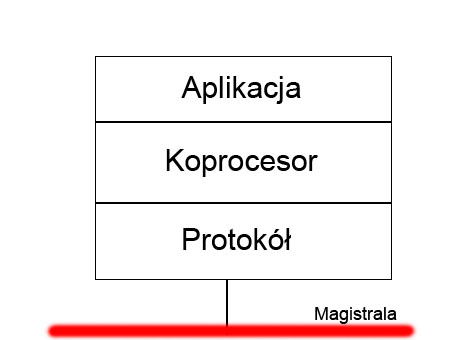
\includegraphics[width=8cm]{./img/wezel.jpg}
\end{center}

\begin{itemize}
	\item Przez \textbf{aplikację} rozumiemy znajdujący się w sterowniku PLC system operacyjny czasu rzeczywistego oraz program cyklicznie realizujący określone przez programistę założenia. Ten poziom odpowiada za faktyczną pracę urządzenia i jest częściowo niezależny od innych węzłów systemu. \\
	\item \textbf{Koprocesor} jest elementem pracującym niezależnie od głównego procesora urządzenia. Jest on odpowiedzialny za komunikację pomiędzy macierzystym układem, a siecią. Posiada dwa zastosowania: 
	\begin{itemize}
		\item \textit{Nadawanie} – otrzymując informacje od procesora głównego,  kopiuje ona odpowiednie fragmenty pamięci do buforów nadawczych, następnie transformuje je do odpowiedniej formy (ramki transmisyjne), po czym wysyła je przy użyciu nadajnika (portu UART) \\
		\item \textit{Odbieranie} – przechwytuje informacje z sieci skierowane do tego węzła i dekoduje je do formy mogącej być odczytaną przez sterownik. Po tym następuje skopiowanie treści do bufora odbiorczego i przepisanie do pamięci urządzenia 
	\end{itemize}
	\item \textbf{Protokół transmisji} jest ściśle związany z koprocesorem sieci. Jest zbiorem zasad, na jakich odbywa się połączenie pomiędzy dwoma lub więcej węzłami w sieci. Dzięki temu możliwa jest komunikacja sterowników działających na różnym oprogramowaniu.\\
	
\end{itemize}

W dalszej części wypracowania skupimy się głównie na protokole transmisji.

\section{\textcolor{blue}{Determinizm czasowy w sieciach przemysłowych}}

Poprzez \textbf{determinizm} działania obiektu (w naszym przypadku węzła sieci) rozumiemy, że dla każdej kombinacji stanu poprzedniego oraz zdarzenia pojawiającego się z zewnątrz, węzeł ten posiada zdefiniowany, jednoznaczny stan pracy. \\
\textbf{Determinizm czasowy} definiujemy jako zgodne z działaniem deterministycznym reakcje obiektu w określonym i skończonym czasie. \\
Można wyróżnić dwa różne rodzaje determinizmu czasowego:
\begin{itemize}
	\item Określony ściśle (ostry), gdzie po upływie określonego czasu od zdarzenia inicjującego $ T_G $ następuje określona reakcja.
	\item Ograniczony granicznie (nieostry) - tutaj reakcja następuje nie później niż do okreslonego czasu $ T_G $.
\end{itemize}
Zależności te można wyrazić poniższymi wzorami:
\begin{itemize}
	\item Determinizm czasowy ściśle określony:
	\begin{equation}
	T_{OS} = T_G
	\end{equation}
	\item Determinizm czasowy granicznie określony
	\begin{equation}
	T_{OS} \leq T_G
	\end{equation}
	\item Dodatkowo:
	\begin{equation}
	T_{OS} = T_R + T_O
	\end{equation}
\end{itemize}
Gdzie
\begin{itemize}
	\item $ T_{OS} $ - czas obsługi sieciowej zdarzenia
	\item $ T_G $ - czas graniczny obsługi
	\item $ T_R $ - czas reakcji na zdarzenie
	\item $ T_O $ - czas właściwej obsługi zdarzenia
\end{itemize}
Determinizm czasowy nie wymaga stuprocentowej niezawodności podczas przekazywania danych. Za poprawną pracę sieci przyjmuje się wtedy sytuację, kiedy nie dochodzi do wystąpienia stanu awaryjnego (zarówno z logicznego, jak i fizycznego punktu widzenia). Najistotniejsze jest, aby czas dostępu do pamięci został obarczony krytycznym czasem granicznym.\\

\section{\textcolor{blue}{Rodzaje protokołów stosowane w sieciach przemysłowych}}

Ponieważ rozproszona sieć przemysłowa czasu rzeczywistego powinna się charakteryzować skończonym czasem przekazywania danych, będą nas interesować jedynie protokoły o zdefiniowanym (deterministycznym) w czasie dostępie. \\
Współcześnie można wyróżnić tylko 3 rodzaje protokołów, które spełniają powyższy warunek:
\begin{itemize}
	\item Token
	\item Master - Slave
	\item Producent - Dystrybutor - Konsument (PDK)
\end{itemize}
Pierwsze dwa protokoły posiadają wiele implementacji i zastosowań, z kolei trzeci z nich jest dość świeży. Wszystkie inne rodzaje protokołów spełniające warunek deterministyczny są pochodnymi lub hybrydami powyższych modeli. \\
Protokół z użyciem Tokena polega na przesyłaniu informacji między równorzędnymi stacjami, posiadającymi dostęp do wspólnej magistrali. Aby zapewnić brak kolizji (sytuacji, w których więcej niż jedna stacja zapisuje dane), stosuje się tzw. żeton (z ang. \textit{Token}). Jest to specjalny rodzaj informacji krążący po sieci od jednej stacji do do drugiej. Odczytanie Tokenu przez węzeł powoduje jej uprzywilejowanie, co w praktyce oznacza prawo do transmisji ramek z danymi. Jednak aby zachować prawo determinizmu czasowego, prawo do zapisu trwa określony czas, a po jego upływie węzeł musi bezwględnie przekazać żeton następnemu użytkownikowi. Token wykorzystywany jest między innymi w protokołach typu Token-Ring (pierścieniowa budowa sieci) i Token-Bus (pojedyncza magistrala, w praktyce konfiguracja gwiazdy). \\
Model PDK bazuje na podziale stacji na 3 rodzaje abonentów: producentów, dystrybutorów oraz konsumentów. "Producent" pełni tu rolę nadawcy: "produkuje" dane, które zostaną użyte przez inne stacje. "Dystrybutor" jest pośrednikiem - jego zadaniem jest transfer danych od producenta (lub wielu producentów) do konsumentów. Dystrybutor przechowuje scenariusz wymian i na jego podstawie określa, kiedy dana informacja ma trafić do sieci. W trakcie podejmowania decyzji, gdzie trafić mają dane pod uwagę brane są średnia konsumpcja oraz aktualne obciążenie konsumentów. "Konsument" to stacja będąca punktem końcowych dla danych, gdzie są one odczytywane i odpowiednio używane. Protokół ten jest używany np. w sieci FIP.


\section{\textcolor{blue}{Sieci o dostępie typu Master-Slave}}
Protokół Master-Slave jest prostą metodą dostępu ze względu na narzucone w niej ograniczenia i sztywne reguły transmisji:
\begin{itemize}
	\item Wymiana informacji jest dopuszczalna jedynie pomiędzy wybraną stację nadrzędną, zwaną Master, a jedną ze stacji podrzędnych, zwanymi Slave
	\item Tylko stacja Master może inicjować transakcje
	\item Dwa rodzaje transmisji:
	\begin{itemize}
		\item \textbf{Zapytanie - Odpowiedź}: polega na wymienia informacji pomiędzy Masterem, a wybraną, konkretną stacją Slave. W tym procesie uczestniczy żądanie (zdefiniowany rozkaz) oraz odpowiedź od Slave.
		\item \textbf{Rozgłoszenie}: żądanie jest wysyłane do wszystkich jednostek Slave w sieci, a Master nie oczekuje od nich odpowiedzi.
	\end{itemize}
	\item Ograniczona liczba rozkazów jaką może realizować Master, czyli ściśle określony zbiór dopuszczalnych wymian
	\item Wymiany informacji odbywają się cyklicznie i nie wymagają ani wstrzymania sieci, ani jej ponownego uruchomienia
\end{itemize}
Powyższe własności sieci Master-Slave niosą ze sobą wiele zalet:
\begin{itemize}
	\item Niskie wymagania z punktu widzenia oprogramowania
	\item Łatwa konfiguracja sieci
	\item Konieczność oprogramowania sprowadza się wyłącznie do koprocesora stacji Master. Stacje Slave mogą wykonywać polecenie sprzętowo, bez konieczności programowania.
	\item Szybkie uruchomienie systemu komunikacyjnego
\end{itemize}


\subsection{Scenariusz wymian}
Scenariusz wymian to szczegółowy opis możliwych wymian danych w sieci. Znajduje się w pamięci koprocesora jednostki Master i jest to jeden z najistotniejszych elementów sieci Master - Slave. Spoczywa na nim obowiązek konfiguracji całej sieci i doprowadzenie do jej sprawnego działania. Struktura scenariusza wymian składa się z listy zmiennych jakie mogą być przesyłane, czyli ich nazw, kierunków transmisji oraz czasów odświeżania.\\
Aby móc wykonać scenariusz wymian wymagane jest zdefiniowanie budowy ramek jakie są przesyłane. Ponieważ w sieci Master - Slave wyróżnia się dwa rodzaje transmisji:
\begin{itemize}
	\item Master - Slave ("żądanie" oraz "rozgłoszenie"), 
	\item Slave - Master ("odpowiedź"), 
\end{itemize}
pojawia się konieczność określenia dwóch typów ramek, gdzie każda będzie mogła wykonać zadanie jednej z transmisji.\\
Elementarną ramkę w tego typu sieci przedstawia poniższa tabela:
\begin{center}
	\begin{tabular}{cccc}
		1 [B] & 1 [B] & n [B] & 2 [B] \\ 
		\hline \multicolumn{1}{|c}{Adres stacji} & \multicolumn{1}{|c}{Kod funkcji} & \multicolumn{1}{|c}{Dane} & \multicolumn{1}{|c|}{Kontrola błędów} \\ 
		\hline 
	\end{tabular}
\end{center}

\begin{itemize}
	\item \textbf{Adres stacji} - określa do której z jednostek Slave należy wysłać dane. Pewna określona wartość w tym polu oznacza "rozgłoszenie", czyli wysłanie ramki do wszystkich stacji Slave, jednak jest ona zależna od rozwiązań firmowych.
	\item \textbf{Kod funkcji} - definiuje rozkaz jaki Master każe wykonać Slave.
	\item \textbf{Dane} - wielkość tego pola jest zależna zarówno od Kodu Funkcji, jak i od konkretnych implementacji sieci. Rola tego pola nie ogranicza się do "surowych" danych, może również zawierać takie informacje jak kod funkcji dodatkowych bądź adres danych, które zależy odczytać.
	\item \textbf{Kontrola błędów} - słowo kontrolne, które ma gwarantować przesył poprawnych danych. Jest zależne od implementacji, może to być m.in. CRC lub LRC.
	\item W zależności od konkretnego rozwiązania, w ramce można wyróżnić jeszcze znaczniki początku ramki oraz końca ramki.
\end{itemize}
Pierwsze dwa pola są identyczne dla obu ramek. W ramce "żądania" w polu Adres Stacji znajduje się albo właściwy adres stacji Slave, bądź Rozgłoszenie. Z kolei w ramce "odpowiedzi" w tym polu może znajdować się albo adres Mastera, albo adres własny ramki - pozwala to Masterowi zweryfikować, czy otrzymana ramka jest od prawidłowej stacji. W polu danych ramki "odpowiedzi" mogą znajdować się albo dane, które są wynikiem wykonania rozkazu, albo jedynie potwierdzenie realizacji. \\\\
Właściwy proces tworzenia scenariusza wymian jest zależny jedynie od upodobań konfigurującego sieć.

\subsection{Dziury w sieci Master - Slave}
\label{subsec:dziury}
"Dziury" są negatywnym zjawiskiem w funkcjonowaniu sieci, które objawia się poprzez przerwę w zbiorze stacji. W sieci Master-Slave źródłem dziur może być wyłącznie uszkodzenie stacji abonenckiej lub jej wyłączenie. Ogółem rzecz biorąc, dziury powstają na wskutek nieobecności stacji w sieci. Skutkiem istnienia dziur jest opóźnienie wymiany informacji pomiędzy Masterem, a stacją podrzędną, co może być niebezpieczne z punktu widzenia krytycznych parametrów sieci, m.in. gwarantowanego czasu dostarczenia informacji. Rolą programistów jest zapewnienie takiej konfiguracji, aby dziury powstawały jak najrzadziej.\\
Prosta topologia sieci Master-Slave oraz nieskomplikowana konfiguracji w postaci scenariusza wymian umożliwiają wykrycie dziur już na wczesnym etapie. Każda wymiana informacji, jaka znajduje się w scenariuszu, jest kierowana wyłącznie do jednego adresata. Jeżeli wystąpi błąd w konfiguracji i wymiana będzie skierowana do nieistniejącego abonenta, zostanie ona wychwycona.\\
Odłączenie lub uszkodzenie stacji Slave może skutkować opóźnieniem czasu pracy, który jest równy sumie czasu transmisji ramki od Mastera oraz czasu oczekiwania na odpowiedź. Co więcej, może się zdarzyć, że do nieaktywnego odbiorcy wysyłana ramka posiada wiele danych i jest bardzo długa, co dodatkowo opóźnia czas reakcji.\\
Jednym z mechanizmów umożliwiających minimalizację strat czasowych związanych z powstawaniem dziur jest określanie liczby cykli w czasie których stacja odbiorcza nie jest odpytywana. Po zakończeniu wszystkich cykli nawiązywana jest próba połączenia ze stacją. Jeżeli i tym razem odbiorca jest nieaktywny, następuje ponowne wstrzymanie wymian z nim oraz odczekanie wcześniej ustalonej liczby cykli. Ta metoda nosi nazwę "autousuwania" nieobecnego abonenta. Zastosowanie tego rozwiązania zależy już wyłącznie od decyzji programisty, który powinien mieć możliwość włączania i wyłączania mechanizmu autousuwania.

\subsection{Parametryzacja wymian}
Parametryzacja jest ważnym elementem programowania koprocesora w stacji Master. Polega na wprowadzeniu przygotowanego scenariusza wymian oraz uzupełnieniu go wymaganymi informacjami.
	\subsubsection{Konfiguracja tablicy wymiany}
	\begin{itemize}
		\item \textbf{Numer wymiany} - jest to niezbędny parametr aby umożliwić zastosowanie mechanizmu wymian wyzwalanych, które są inicjowane przez aplikację. Liczba wymian w pojedynczym cyklu jest zależna od programisty i w zależności od konkretnej implementacji sieci, może osiągnąć nawet kilkaset.
		\item \textbf{Numer abonenta} - określa do której ze stacji Slave wymiana jest kierowana.
		\item \textbf{Kod operacji}
		\item \textbf{Adres pobrania danych} - definiuje miejsce w pamięci jednostki centralnej Master, które będzie źródłem danych.
		\item \textbf{Adres przesłania danych} - definiuje miejsce w jednostce centralnej stacji Slave, gdzie zostaną przekazane dane.
		\item \textbf{Liczba danych}
		\item \textbf{Wybór trybu przesłania} - może być \textit{periodyczny}, czyli wymiana wykonuje się w każdym cyklu pracy sieci, lub \textit{wyzwalany}, czyli wymiana realizowana jest przez program jednostki centralnej.
		\item \textbf{Autousuwanie} - określa czy przy braku odpowiedzi ze strony abonenta zostaje uruchamiany ten mechanizm. Został opisany w poprzednim podrozdziale.
		\item \textbf{Adres słowa raportu wymiany z daną stacją}
	\end{itemize}
	\subsubsection{Konfiguracja tablicy parametrów wymiany}
	Dla każdej wymiany z osobna należy wypełnić jej tablice parametrów, na którą składają się m.in.:
	\begin{itemize}
		\item Maksymalny czas oczekiwania na odpowiedź od stacji Slave $ T_{OD} $ - bardzo ważny parametr, którego wartość powinna być wynikiem dokładnej analizy obciążenia sieci (w szczególności czas pracy abonenta oraz czas trwania cyklu jego jednostki centralnej $ T_{A} $).
		\item Liczba prób nawiązania łączności z abonentem - określa maksymalną liczbę prób nawiązania połączenia w przypadku braku odpowiedzi ze strony stacji Slave. Ma wielki wpływ na przepustowość sieci oraz zjawisko powstawania "dziur" [~\ref{subsec:dziury}~].
		\item Maksymalna liczba cykli przy braku odpowiedzi - w czasie trwania tych cykli nie będzie prób nawiązania komunikacji ze stacją Slave, którą wykryto jako nieobecną. Ten parametr również został opisany w podrozdziale dotyczącym zjawisko "dziur" [~\ref{subsec:dziury}~].
		\item Przerwa czasowa między dwiema transakcjami typu "rozgłoszenie" (\emph{broadcast}).
		\item Czas opóźnienia występujący przed oraz po transmisji ramki.
		\item Czas autoryzacji w przypadku pracy z modemami.
	\end{itemize}
	\subsubsection{Parametry globalne}
	Istnieje pewna część parametrów, które muszą zostać zdefiniowane globalnie, tzn. nadrzędnie dla każdej wymiany w sieci. Wszystkie wymiany muszą pracować zgodnie z nimi aby umożliwić prawidłową pracę sieci.
	\begin{itemize}
		\item Tryb transmisji, w przypadku sieci Modbus można wyróżnić:
		\begin{itemize}
			\item RTU - transmisję bitową
			\item ASCII - transmisję znakową
		\end{itemize}
		Tryby transmisji nie mogą być mieszane i w czasie trwania transakcji należy zachować tylko jeden z nich. Nie każdy protokół oparty na Master-Slave posiada kilka trybów, np. Magistrala LIN.
		\item Liczba bitów stopu
		\item Rodzaj kontroli parzystości
		\item Liczba bitów definiująca pojedynczy znak transmisji $ L_{BZ} $
		\item Szybkość transmisji $ V $
	\end{itemize}
\newpage
	\subsection{Zjawiska zachodzące pomiędzy koprocesorem, a jednostką centralną}
	Analiza procesów zachodzących na styku "koprocesor - jednostka centralna" jest naturalną koniecznością wynikającą z programowania i parametryzacji wymian w sieci. Jest to niezbędne aby precyzyjnie wyznaczyć dwa bardzo istotne parametry związane z konfiguracją sieci:
	\begin{itemize}
		\item $ T_{OD} $ - czas oczekiwania stacji Master na odpowiedź od stacji Slave
		\item $ T_{GOT} $ - czas oczekiwania na gotowość jednostki centralnej stacji Slave
	\end{itemize}
	W pierwszej kolejności należy określić parametr $ T_{GOT} $, który ma umożliwić stacji Slave spokojne wykonanie powierzonych jej zadań. Parametr ten może zostać ustawiony albo globalnie dla wszystkich stacji Slave, albo lokalnie dla każdej z nich. Wówczas każdy z abonentów posiada indywidualną wartość $ T_{GOT_j} $, zależną od jego potrzeb. Sam parametr można zdefiniować następującym wzorem (indeks dolny \emph{i} oznacza parametr stacji Master, natomiast \emph{j} parametr jednej ze stacji Slave):
	$$ T_{GOT_j} = T_{DR} + \max{(T_{AR_j})} + \max{( T_{A_j} )} + \max{( T_{PR_j} )} $$
	Gdzie:
	\begin{itemize}
		\item $ T_{DR} $ \tab\tab{- czas detekcji ramki}
		\item $ \max{(T_{AR_j})} $ \tab{- maksymalny czas analizy ramki}
		\item $ \max{( T_{A_j} )} $ \tab{- maksymalny czas trwania cyklu pracy w stacji Slave}
		\item $ \max{( T_{PR_j} )} $ \tab{- maksymalny czas przygotowania ramki odpowiedzi przez stację Slave}
	\end{itemize}
	Innymi słowy, największy dopuszczalny parametr $ T_{GOT} $ oznacza maksymalny czas jaki jest potrzebny co najmniej jednej ze stacji Slave na wykrycie ramki od stacji Master, jej poprawne przetworzenie i udzielenie odpowiedzi.\\
	W drugiej kolejności należy określić parametr $ T_{OD} $, który powinien być większy od największej wartości $ T_{GOT} $ i jednocześnie powiększony o czas wykonywania wszystkich czynności niezbędnych do wysłania ramki żądania z stacji Master oraz odebrania ramki odpowiedzi ze stacji Slave. Możemy zatem $ T_{OD} $ zdefiniować następująco:
	$$ T_{OD}=\max{(T_{GOT_j}+ T_{PR_i}+T_{TR_i}+T_{TR_j}+T_{DR}+T_{AR_i}+T_{A_i})} $$
	Gdzie:
	\begin{itemize}
		\item $ T_{GOT_j} $ \tab{- największy czas $ T_{GOT} $ spośród czasów stacji Slave}
		\item $ T_{PR_i} $ \tab{- czas przygotowania ramki żądania}
		\item $ T_{TR_i} $ \tab{- maksymalny czas transmisji ramki żądania}
		\item $ T_{TR_j} $ \tab{- maksymalny czas transmisji ramki odpowiedzi o największej możliwej długości}
		\item $ T_{DR} $ \tab{- czas detekcji ramki odpowiedzi}
		\item $ T_{AR_i} $ \tab{- maksymalny czas analizy ramki odpowiedzi}
		\item $ T_{A_i} $ \tab{- maksymalny czas trwania cyklu pracy w stacji Master}
	\end{itemize}
	Zastosowanie powyższych wzorów daje gwarancję, że w sieci Master - Slave każda transakcja zostanie poprawnie wykonana, jednak wartości te będą wpisane odgórnie oraz, ponieważ uwzględniają najgorsze możliwe przypadki, transakcje, które mogłyby wykonać się krócej, będą trwać tak samo długo jak inne. Czas ten można zmniejszyć posługują się mechanizmem autousuwania, ale należy korzystać z niego z rozwagą.
\newpage
	\subsection{Czas trwania cyklu sieci}
	Jest to niezwykle ważny parametr, który określa czas nadawania pomiędzy stacjami, jak również możliwości sieci do wykonywania określonych zadań.\\
	Aby móc przystąpić do określenia tego czasu potrzebne są pewne założenia i uproszczenia:
	\begin{itemize}
		\item W omawianej sieci nie występuje zjawisko "dziur" [~\ref{subsec:dziury}~]
		\item Znany jest scenariusz wymian - w sieci istnieje \emph{N} wymian
		\item Znane są długości wszystkich ramek
	\end{itemize}
	Przystępujemy zatem do analizy naszej sieci:
	\begin{enumerate}
		\item Czas transmisji pojedynczej ramki
		\begin{equation}
			T_{TR}=\cfrac{[LZT] \cdot [LBZ]+[BS]}{V}
		\end{equation}
		Gdzie:
		\begin{itemize}
			\item \emph{LZT} \tab{- liczba znaków transmisji}
			\item \emph{LBZ} \tab{- liczba bitów w pojedynczym znaku}
			\item \emph{BS} \tab{- liczba bitów sterujących}
			\item \emph{V} \tab{- prędkość transmisji transmisji}
		\end{itemize}
		\item Czas transmisji ramki żądania wysyłanej przez stację Master
		\begin{equation}
			T_{TR_i}=\cfrac{[LZT_i] \cdot [LBZ]+[BS]}{V}
		\end{equation}
		\item Czas transmisji ramki odpowiedzi wysyłanej przez stację Slave
		\begin{equation}
			T_{TR_j}=\cfrac{[LZT_j] \cdot [LBZ]+[BS]}{V}
		\end{equation}
		\item Z tymi danymi można przystąpić do obliczenia czasu pojedynczej wymiany, która jest równa sumie czasów wysłania i wykonania żądania, przesłania i odebrania odpowiedzi oraz analizy i wpisu wyniku transakcji:
		\begin{equation}
			T_{W_{i}} = \underbrace{T_{PR_i} + T_{TR_i}}_{T_{Zi}} +
			\underbrace{T_{DR}+T_{AR_j}+T_{A_j}+T_{PR_j}+T_{TR_j}}_{T_{T_{Oj}}} + 
			\underbrace{T_{DR}+T_{AR_i}+T_{A_i}}_{T_{RA_i}}
		\end{equation}
		Gdzie:
		\begin{itemize}
			\item $ T_{Zi} $ \tab{- czas emisji żądania, składa się z czasów przygotowania i transmisji ramki żądania}
			\item $ T_{Oj} $ \tab{- czas emisji odpowiedzi, składa się z czasów detekcji i analizy ramki żądania, przygotowania i transmisji ramki odpowiedzi oraz czasu oczekiwania na sygnał końca dla stacji Slave}
			\item $ T_{RA_i} $ \tab{- czas analizy i wpisu wyniku wymiany, składa się z czasów wykrycia i analizy ramki oraz czasu oczekiwania na sygnał końca dla stacji Master}
		\end{itemize}
		\item Teraz wystarczy ten czas przenieść na wykonania \emph{N} wymian w sieci:
		\begin{align}
			T_{CW} &= \sum_{i=1}^{N}{T_{W_i}}=
			\sum_{i=1}^{N}{{T_{PR_i} + T_{TR_i}}} + 
		 	\sum_{i=j}^{N}{T_{AR_j}+T_{A_j}+T_{PR_j}+T_{TR_j}} \nonumber \\
			&\qquad {} + \sum_{i=1}^{N}{T_{AR_i}+T_{A_i}} +
			2\cdot N\cdot T_{DR}
		\end{align}
		\item Powyższy czas może się zwiększyć jeżeli w sieci będą występować "dziury", które skutkują powtarzaniem wymian (repetycji). Dla $ N_R $ powtarzanych transmisji w całym scenariuszu wymian (realizacja wymian periodycznych) w najgorszym możliwym przypadku dodatkowy czas wyniesie:
		\begin{equation}
			T_{REP} = \sum_{i=1}^{N}{N_{R_i}\cdot T_{TR_i}+N_R\cdot T_{OD_i}}
		\end{equation}
		Gdzie:
		\begin{itemize}
			\item $ T_{TR_i} $ \tab{- czas transmisji żądania dla \emph{i}-tego powtórzenia}
			\item $ N_{R_i} $ \tab{- liczba powtórzeń do \emph{i}-tego abonenta}
			\item $ N $ \tab{- liczba abonentów}
			\item $ T_{OD_i} $ \tab{- czas czekania na odpowiedź przez stację Master}
		\end{itemize}
		\item Zatem łączny czas trwania cyklu powiększony o czas realizacji repetycji jest równy:
		\begin{equation}
			T_{W_{MAX}}=T_{CW}+T_{REP}
		\end{equation}
		\item Na koniec należy jeszcze uwzględnić realizację wymian wyzwalanych. Ten kolejny dodatkowy czas jest całkowicie zależny od rozwiązań firmowych - należy znać liczbę wymian wyzwalanych oraz postacie ich funkcji.\\
		Zakładając, że w sieci realizowana jest tylko jeden rodzaj wymiany wyzwalanej oraz w jednym cyklu pracy zostanie zrealizowanych $ N_W $ takich wymian, czas zwiększy się dokładnie o $ N_W $ cykli aplikacji, które je uruchomiła. Wówczas czas zwiększa się o:
		\begin{equation}
			T_{WW} = N_W\cdot T_{A_j} + \sum_{i=1}^{N_W}{T_{W_i}}
		\end{equation}
		Gdzie:
		\begin{itemize}
			\item $ T_{A_j} $ \tab{- czas oczekiwania na sygnał końca dla stacji Slave}
			\item $ T_{W_i} $ \tab{- czas wykonania \emph{i}-tej wymiany wyzwalanej}
		\end{itemize}
		\item Ostatecznie wzór na czas trwania cyklu sieci przyjmuje postać:
		\begin{equation}
			T_{W_{MAX}}=T_{CW}+T_{REP}+T_{WW}
		\end{equation}
		Gdzie $ T_{CW} $ oznacza czas trwania cyklu dla bezbłędnie działającej sieci, a $ T_{REP} $ oraz $ T_{WW} $ określają potencjalny nakład czasowy.
	\end{enumerate}



	\subsection{Sprawność sieci i jej przepustowość}
	Znając całkowity czas pojedynczej transakcji danych ze wzoru \textit{(4)}, można przystąpić do wyliczenia wartości określających efektywność czasową przesyłania danych w sieci:
	\begin{itemize}
		\item \textbf{Sprawność} wyznacza stosunek czas przesyłu danych do całkowitego przesyłu danych w transakcji. Liczona w procentach.
		\item \textbf{Przepustowość} pozwala określić maksymalną ilość informacji, jaka zostanie przesłana w jednostce czasu. Liczona w bitach na sekundę.
	\end{itemize}
	
	Wartości te przedstawia się za pomocą poniższych wzorów
	\begin{equation}
	\eta = \cfrac{\cfrac{8\cdot n}{V}}{T_{Wi}}   
	\end{equation}
	\begin{equation}
	P = \cfrac{8\cdot n}{T_{Wi}}
	\end{equation}
	
	Gdzie:
	\begin{itemize}
		\item η - sprawność
		\item P - przepustowość
		\item n - liczba bajtów danych
		\item V - szybkość transmisji danych w siecie
		\item $ T_{Wi} $ - Całkowity czas trwania pojedynczej transkacji danych (wliczająć ramkę żądania)
	\end{itemize}
	
	Ponieważ wartość $ T_{Wi} $ nie jest stałą zdefiniowaną globalnie, a indywidualną dla każdej ramki, wartości obu wielkości można wyrazić za pomocą przedziałów, używając w tym celu minimalnego i maksymalnego czasu trwania transakcji danych. \\
	W praktyce dość często sprawność i przepustowość obliczana jest po odrzuceniu narzutu czasowego powstałego w wyniku dodatkowych akcji na magistrali, nie będących transmisją danych, m. in. czasu detekcji $ T_{DR} $ czy czasu transmisji tamki żądania $ T_{TR_i} $. W tym celu w miejsce $ T_{Wi} $ podstawiamy równanie ze wzoru \textit{(1)}. Po zamianie uzyskuje się nowe wartości, obejmujące wyłącznie czasu transakcji danych.
	
	\begin{equation}
	\eta = \cfrac{\cfrac{8\cdot n}{V}}{\cfrac{[LZT] \cdot [LBZ]+[BS]}{V}} = \cfrac{8\cdot n}{[LZT] \cdot [LBZ]+[BS]}
	\end{equation}
	\begin{equation}
	P = \cfrac{8\cdot n}{\cfrac{[LZT] \cdot [LBZ]+[BS]}{V}} = \cfrac{8\cdot n \cdot V}{[LZT] \cdot [LBZ]+[BS]}
	\end{equation}
	
		
	\subsection{Możliwości optymalizacji}
	
	Niezależnie od stosowanego podejścia, sprawność i przepustowość rośnie wraz z długością ramki. Należy jednak pamiętać, że jej zwiększanie niesie ze sobą również skutki uboczne - rośnie czas transmisji oraz cykl przetwarzania (co z kolei zwiększa czas trwania cyklu sieci). \\
	W celu polepszenia parametrów czasowych, przede wszystkim powinno się poprawić czas trwania wymian - jest to najbezpieczniejszy sposób usprawnienia przepustowości i sprawności sieci (nie licząc zmiany sterównik i/lub koprocesorów na ich szybsze odpowiedniki). Optymalizacja powinna dotyczyć zwłaszcza jednostki nadrzędnej Master, ponieważ jest on inicjatorem lub odbiorcą każdej transakcji w systemie. Usprawnienie działania koprocesorów stacji Slave również poprawia parametry czasowe, lecz opatrzone jest mniejszym priorytetem. \\
	Można wyodrębnić kilka zasad, które pozwalają na usprawnienie działania sieci:
	\begin{itemize}
		\item Skrócenie czasu trwania cyklu jednostki Master - można to uzyskać np. za pomocą podziału programu sterownika na mniejsze fragmenty, by zwiększyć częstotliwość komunikacji jednostki centralnej z koprocesorem.
		\item W przypadku, kiedy Master kilkakrotnie wymienia informacje z tą samą jednostką podrzędną, można zrezygnować z raportu wymiany. Następuje wtedy grupowanie i wysłanie jednego raportu w ramach grupy zamiast pojedynczego dla każdej zrealizowanej transakcji.
		\item Innym sposobem jest grupowanie danych przeznaczonych dla tego samego Slave'a już w jednostce centralnej Mastera, a następnie wysłanie ich w jednej, dłuższej ramce.
		\item Wysyłanie jak największej liczby informacji w trakcie wymian wyzwalanych - najlepiej, aby były to sporadycznie używane polecenia, lub dane o mniejszym priorytecie. Ponieważ wymiany wyzwalane są stosowane rzadziej w porównaniu do cyklicznych, sieć zostanie odciążona z niepotrzebnych, nadmiarowych wymian. Dodatkowo, uzyskamy więcej miejsca na pilne transakcje.
		\item Należy zadbać, aby wymiany cykliczne z tym sam abonentem nie następywały zaraz po sobie - po każdej transakcji Slave potrzebuje odrobiny czasu, aby zidentyfikować (zinterpretować) polecenie od arbitra sieci, skomunikować się ze swoją jednostką centralną oraz stworzyć odpowiedź.
		\item Szczególny przypadek powyższego punktu: jeżeli do jednej stacji podrzędnej wysyłany jest rozkaz zapisu i odczytu, to wpierw należy dokonać odczytu danych, a następnie zapisu. Taka kombinacja jest szybsza o jeden cykl jednostki centralnej Slave'a dla każdej takiej pary.
	\end{itemize}


\newpage
\begin{thebibliography}{2}
	\bibitem{Hab} Andrzej Kwiecień, \textit{Analiza przepływu informacji w komputerowych sieciach przemysłowych}, Gliwice 2002
	\bibitem{RS} Wojciech Mielczarek, \textit{Szeregowe interfejsy cyfrowe}, Helion, Gliwice 1997
	\bibitem{tcp} Piotr Gaj, \textit{Zastosowanie protokoły TCP/IP do transmisji informacji dla potrzeb przemysłowych systemów kontrolno-nadzorczych. Rozprawa dokotroska.}, Gliwice, 2003
\end{thebibliography}

\end{document}